\def\t#1{\texttt{#1}}
\def\h#1{{\tt \color{gray} #1}}
\def\swf{\h{"<s>"}}
\def\maxAmb#1{$\langle \Sigma \rangle_#1$}
\def\maxAmbFSA#1{$\langle \Sigma,S \rangle_#1$}
\def\maxAmbCFG#1{$\langle \Sigma,\Sigma^{\prime} \rangle_#1$}
\def\exampleWord{{present}}


\section{Generative Constraint Grammar}
\label{sec:expressivity}

Symbolic sentences have an attractive side effect: they let us model
CG as a generative formalism. This section is a detour from the
central theme of analysis and quality control of natural language
grammars; the uninterested or time-constrained reader may well skip it.

We view a constraint grammar CG as generating a formal language $\mathcal{L}$
over an alphabet $\Sigma$ as follows.
We encode words $w \in \Sigma^\star$ as a sequence of cohorts, each of which has
one of the symbols of $w$ as a reading.
A constraint grammar CG rejects a word if, when we pass its encoding through the
CG, we get back the cohort \t{"<REJECT>"}. A constraint grammar CG accepts a word
if it does not reject it.
We generate the language $\mathcal{L}$ by passing every $w \in \Sigma^\star$
through the CG, and keeping those which are accepted.

As an example, consider the language $a^\star$ over $\Sigma = \{a,b\}$.
This language is encoded by the following constraint grammar:
\begin{center}
  \begin{Verbatim}
    LIST A = "a";
    LIST B = "b";
    SET LETTER = A OR B;
    SELECT A;
    ADDCOHORT ("<REJECT>")
        BEFORE LETTER 
        IF (-1 (>>>) LINK 1* B);
    REMCOHORT LETTER
  \end{Verbatim}
\end{center}
We then encode the input words as a series of letter cohorts with readings
(e.g.\ \(\t{"<l>"}\;\t{"a"}\), \(\t{"<l>"}\;\t{"b"}\)), and run the grammar.
For instance, if we wished to know whether either word in $\{aaa,aab\}$ is part
of the language $a^\star$, we would run the following queries:
\begin{center}
  \begin{tabular}{l|c}
    \textbf{Input}         & \textbf{Output} \\ \hline
    \(\t{"<l>"}\;\t{"a"}\) & \(\t{"<l>"}\;\t{"a"}\) \\
    \(\t{"<l>"}\;\t{"a"}\) & \(\t{"<l>"}\;\t{"a"}\) \\
    \(\t{"<l>"}\;\t{"a"}\) & \(\t{"<l>"}\;\t{"a"}\) \\ \hline
    \(\t{"<l>"}\;\t{"a"}\) & \t{"<REJECT>"} \\
    \(\t{"<l>"}\;\t{"a"}\) \\
    \(\t{"<l>"}\;\t{"b"}\)
  \end{tabular}
\end{center}
As CG is a tool meant for disambiguation, we can leverage its power to run both
queries at once:
\begin{center}
  \begin{tabular}{l|c}
    \textbf{Input}                  & \textbf{Output} \\ \hline
    \(\t{"<l>"}\;\t{"a"}\)          & \(\t{"<l>"}\;\t{"a"}\) \\
    \(\t{"<l>"}\;\t{"a"}\)          & \(\t{"<l>"}\;\t{"a"}\) \\
    \(\t{"<l>"}\;\t{"a"}\;\t{"b"}\) & \(\t{"<l>"}\;\t{"a"}\)
  \end{tabular}
\end{center}
This is a powerful feature, because it allows us disambiguate based on some
formal language $\mathcal{L}$ if we can find the CG which generates it.
However, the limitations of this style become apparent when we look at a run of
a CG for the language $\{ab,ba\}$:
\begin{center}
  \begin{tabular}{l|c}
    \textbf{Input}                  & \textbf{Output} \\ \hline
    \(\t{"<l>"}\;\t{"a"}\;\t{"b"}\) & \(\t{"<l>"}\;\t{"a"}\;\t{"b"}\) \\
    \(\t{"<l>"}\;\t{"a"}\;\t{"b"}\) & \(\t{"<l>"}\;\t{"a"}\;\t{"b"}\) \\
  \end{tabular}
\end{center}
While the output contains the interpretations $ab$ and $ba$, it also includes
$aa$ and $bb$. Therefore, while this style is useful for disambiguating using
CGs based on formal languages, it is too limited to be used in defining the
language which a CG generates.
% Wen:
%   We should include a reference to the other formalism here, or to the
%   discussion section in which we talk about the disjunction problem.
% Inari:
%   Yeah, I am wondering myself too what's the best place to talk about it.
%   Maybe it becomes easier when we have more pages to fill? 

In light of the idea of using CGs based on formal languages for disambiguating,
it seems at odds with the philosophy of CG to reject by replacing the entire
input with a single \t{"<REJECT>"} cohort. 
%CG generally refuses to remove the
%last possible reading of a cohort, under the philosophy that \emph{some}
%information is certainly better than none.
However, for the definition of CG as a formal language, we need some sort of
distinctive output for rejections. Hence, we arrive at \emph{two} distinct ways
to run generative CGs: the method in which we input unambiguous strings, and
output \t{"<REJECT>"}, which is used in the definition of CG as a formal
language; and the method in which we input ambiguous strings, and simply
disambiguate as far as possible. 


It should be noted that VISL CG-3 \cite{bick2015,vislcg3} supports
commands such as \t{EXTERNAL}, which runs an external executable. It
should therefore be obvious that the complete set of VISL CG-3
commands, at least theoretically, can generate any recursively
enumerable language. For this reason, we will investigate particular
subsets of the commands permitted by CG.  In
sections~\ref{sec:lowerbound} and~\ref{sec:regular}, we will restrict
ourselves to the subset of CG which only uses the \t{REMOVE} command
with sections, and show this to at least cover all regular languages
and some context-free and context-sensitive languages.  In the
original article \cite{kokke2017expressivity}, we address more subsets
and complexity classes.

\begin{figure}[h]
  \centering
  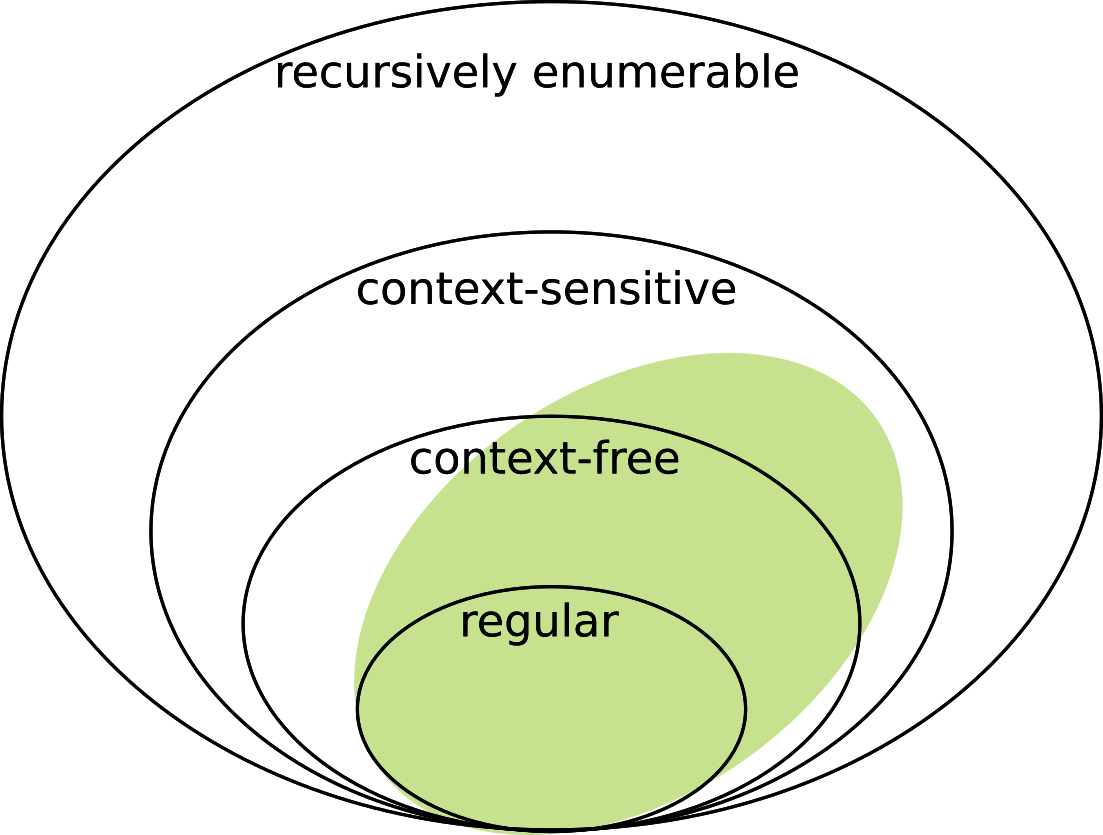
\includegraphics[width=0.4\linewidth]{chapters/chomsky}
  \caption{Lower bound on the expressivity of the subset of CG using only \t{REMOVE}.}
  \label{fig:nocorr}
\end{figure}

\subsection{A lower bound for CG}\label{sec:lowerbound}
In this section, we will only use the \t{REMOVE} command with sections, in
addition to a single use of the \t{ADDCOHORT} command to add the special cohort
\t{"<REJECT>"}, and a single use of the \t{REMCOHORT} command to clean up
afterwards. 
We show that, using only these commands, CG is capable of generating some
context-free and context-sensitive languages, which establishes a lower bound on 
the expressivity of CG (see Figure~\ref{fig:nocorr}).


\paragraph{Example grammar: $a^nb^n$}
Below, we briefly describe the CG which generates the language $a^nb^n$.
This CG is defined over the alphabet $\Sigma$, in addition to a hidden alphabet
$\Sigma^\prime$. These hidden symbols are meant to serve as a simple form of
memory. When we encode our input words, we tag each cohort with \emph{every}
symbol in the hidden alphabet\footnote{
  We can automatically add these hidden symbols to our cohorts using a single
  application of the \t{ADD} command.
}, e.g.\ for some symbol $\ell \in \Sigma$ and $\Sigma' = \{h_1,\dots,h_n\}$ we
would create the cohort \(\t{"<\(\ell\)>"}\;\t{"h\(_1\)"}\;\dots\;\t{"h\(_n\)"}\).

The CG for $a^nb^n$ uses the hidden alphabet \{\t{odd}, \t{even}, \t{opt\_a},
\t{opt\_b}\}. These symbols mean that the cohort they are attached to is in an
even or odd position, and that $a$ or $b$ is a legal option for this cohort,
respectively. The CG operates as follows: 
\begin{enumerate}
\item
  Is the number of characters even? We know the first cohort is odd, and the
  rest is handled with rules of the form \t{REMOVE even IF (NOT -1 odd)}. If the
  last cohort is odd, then discard the sentence. Otherwise continue\dots
\item
  The first cohort is certainly $a$ and last is certainly $b$, so we can
  disambiguate the edges: 
  \t{REMOVE opt\_b IF (NOT -1 (*))}, and \t{REMOVE opt\_a IF (NOT 1 (*))}. 
\item
  Disambiguate the second cohort as $a$ and second-to-last as $b$, the third as
  $a$ and third-to-last as $b$, etc, until the two ends meet in the middle. If
  every \t{"<a>"} is marked with \t{opt\_a}, and every \t{"<b>"} with
  \t{opt\_b}, we accept. Otherwise, we reject.  
\end{enumerate}
The language $a^nb^n$ is context-free, and therefore CG must at least partly
overlap with the context-free languages.


\paragraph{Example grammar: $a^nb^nc^n$}
We can extend the approach used in the previous grammar to write a grammar which
accepts $a^nb^nc^n$. Essentially, we can adapt the above grammar to find the
middle of any input string. Once we have the middle, we can ``grow'' $a$s from
the top and $b$s up from the middle, and $b$s down from the middle and $c$s up
from the bottom, until we divide the input into three even chunks.
If this ends with all \t{"<a>"}s marked with \t{opt\_a}, all \t{"<b>"}s marked
with \t{opt\_b}, and all \t{"<c>"}s marked with \t{opt\_c}, we accept.
Otherwise, we reject.

The language $a^nb^nc^n$ is context-sensitive, and therefore CG must at least
partly overlap with the context-sensitive languages.

\begin{figure}[h]
  \centering
  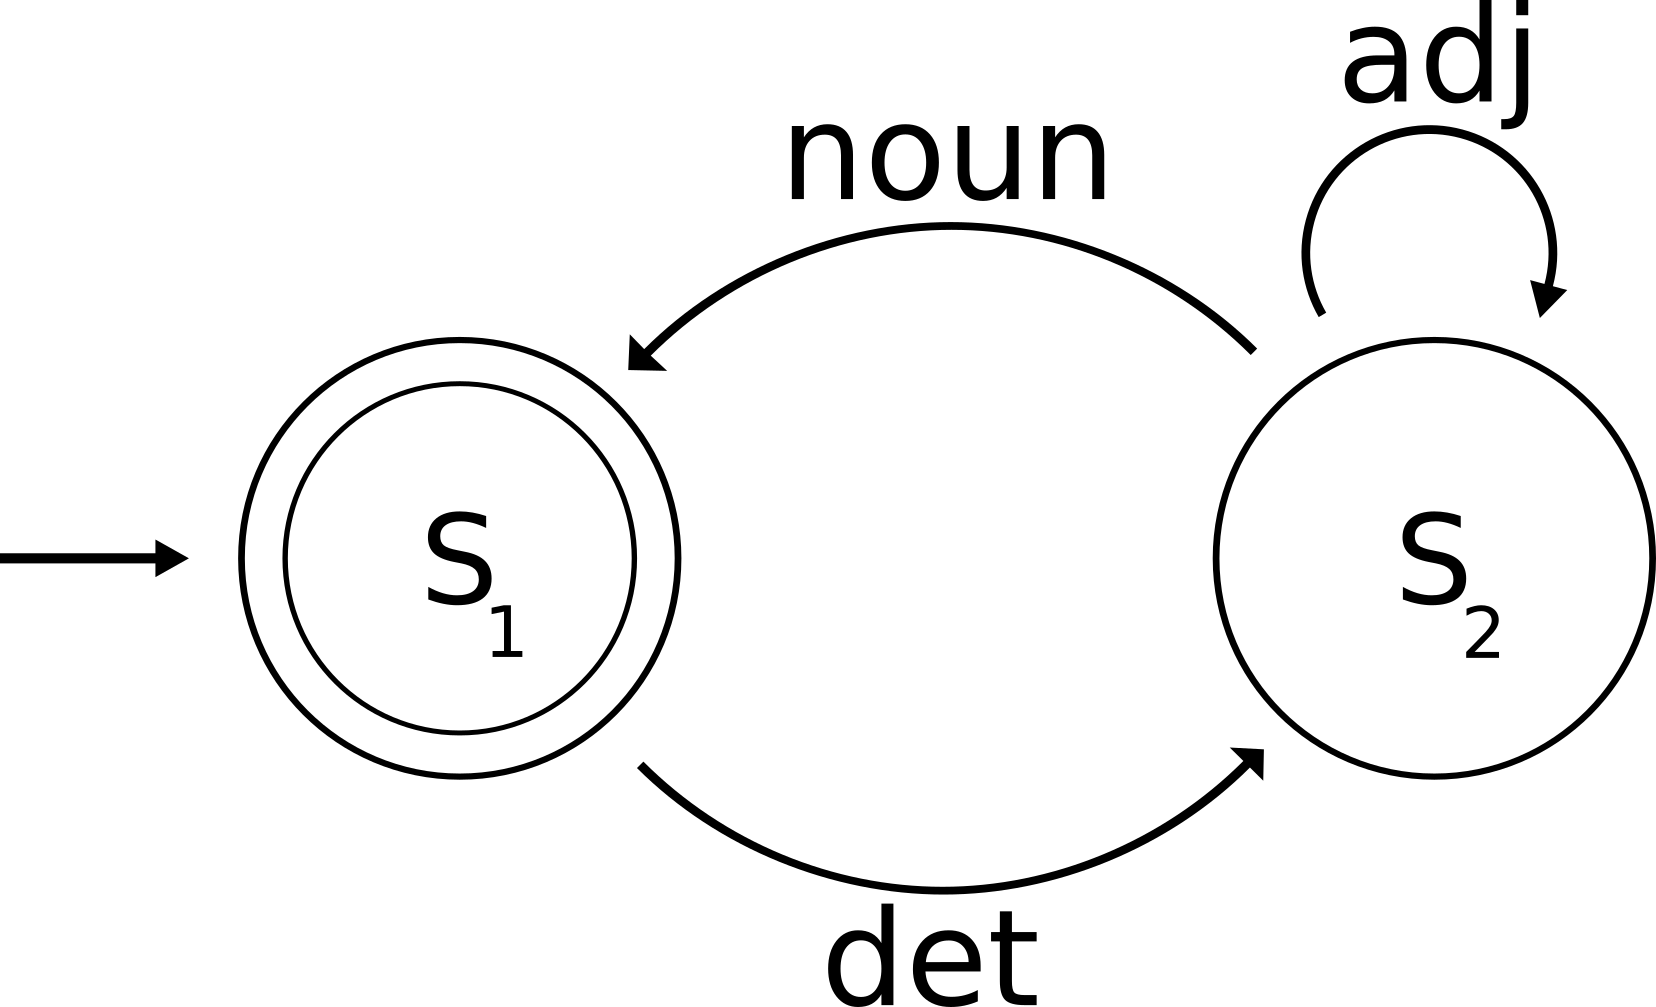
\includegraphics[width=0.4\linewidth]{chapters/fsa.png}
  \caption{A finite-state automaton describing the regular language \t{det
      (adj)* noun}.}
 \label{fig:fsa}
\end{figure}

\subsection{CG is regular}\label{sec:regular}
In the present section, we propose a method to transform arbitrary
finite-state automata into CG. We show how any finite-state automaton
can be expressed in a CG: encode the states and transitions as
ambiguous cohorts, and the disambiguated result shows both the correct
sequence and its path in the automaton.  The translation is
implemented in Haskell, and can be found on GitHub\footnote{See
  \url{https://github.com/inariksit/cgexp}}.



\paragraph{Finite-state automata}
Formally, a finite-state automaton is a 5-tuple
\[
  \langle \Sigma, S, s_0, \delta, F \rangle.
\]


\noindent $\Sigma$ is the alphabet of the automaton, $S$ is a set of states,
including a starting state $s_0$ and a set $F$ of final states.
$\delta$ is a transition function, which takes one state and one
symbol from the alphabet, and returns the state(s) where we can get
from the original state with that symbol.
The automaton in Figure~\ref{fig:fsa} is presented as follows:

\[\!
\begin{aligned}
  &S&      \!\!\!\!=\;& \{\t{s1}, \t{s2}\}  &&\Sigma& \!\!\!\!=\;& \{\emph{det, adj, n}\} \\
  &s_0&    \!\!\!\!=\;& \t{s1}              &&\delta& \!\!\!\!=\;& \{\t{s1} \xrightarrow{\text{\em det}} \{\t{s2}\},  \\ 
  &F&      \!\!\!\!=\;& \{\t{s1}\}          &&      & \!\!\!\! \;& \ \t{s2} \xrightarrow{\text{\em adj}} \{\t{s2}\}, \\
  & &                 &                     &&      & \!\!\!\! \;& \ \t{s2} \xrightarrow{\text{\em noun}} \{\t{s1}\} \} \\
\end{aligned}
\]

Informally, the automaton describes a simple set of possible noun
phrases: there must be one determiner, one noun, and 0 or more
adjectives in between. 
We implement a corresponding CG in the following sections.


\paragraph{Cohorts and sentences}

We encode our input as a sequence of \emph{state cohorts} and \emph{transition cohorts}.
Initially, a state cohort contains the full set $S = \{\t{s1}, \t{s2}\}$ as
its readings, and a transition cohort contains the alphabet $\Sigma =
\{\emph{det, adj, noun}\}$, or some subset of it. As an example, we
generate all 2-letter words recognised by the automaton in
Figure~\ref{fig:fsa}. The initial maximally ambiguous input for length
2 looks as follows:
%
\begin{center}
  \renewcommand{\tabcolsep}{2.5pt}
  \begin{tabular}{ccccc}
    \swf   & \t{"<w>"}  & \swf   & \t{"<w>"} & \swf   \\ 
    \h{s1} & \t{det}      & \h{s1} & \t{det} & \h{s1} \\
    \h{s2} & \t{adj}      & \h{s2} & \t{adj} & \h{s2} \\
           & \t{noun}     &        & \t{noun} &               
  \end{tabular}
\end{center}
%
\noindent 
The grammar disambiguates both transition cohorts and state cohorts. Thus
the desired result shows both the accepted sequence(s)---\emph{det noun}
in this case---and their path(s) in the automaton.
%
\begin{center}
  \renewcommand{\tabcolsep}{2.5pt}
  \begin{tabular}{ccccc}
    \swf   & \t{"<w>"}  & \swf   & \t{"<w>"} & \swf   \\ 
    \h{s1} & \t{det}    & \h{s2} & \t{noun}  & \h{s1}       
  \end{tabular}
\end{center}
%
We can easily adapt the disambiguation scheme for real-world
ambiguities, such as ``the \exampleWord{}''. The state cohorts are identical, but the transition
cohorts contain now some actual word form, and the initial ambiguity
is not over the whole $\Sigma$, but some subset of it.
%
\begin{center}
  \renewcommand{\tabcolsep}{2.5pt}
  \begin{tabular}{ccccc}
    \swf   & \t{"<the>"}  & \swf   & \t{"<\exampleWord{}>"} & \swf    \\ 
    \h{s1} & \t{det}      & \h{s1} & \t{adj}   & \h{s1}  \\
    \h{s2} &              & \h{s2} & \t{noun}  & \h{s2}     
  \end{tabular}
\end{center}
%
The disambiguation process goes exactly like in the first version, with full
$\Sigma$ in the transition cohorts.
Depending on how much the initial input contains ambiguity, the
result may be the same, or more disambiguated. For our example, the
output is identical.
\begin{center}
  \renewcommand{\tabcolsep}{2.5pt}
  \begin{tabular}{ccccc}
    \swf   & \t{"<the>"}  & \swf   & \t{"<\exampleWord{}>"} & \swf    \\ 
    \h{s1} & \t{det}      & \h{s2} & \t{noun} & \h{s1}  \\
  \end{tabular}
\end{center}
%
%
\paragraph{Rules}
Given that every transition happens between two states, and every state 
has an incoming and outgoing transition, every rule needs only
positions -1 and 1 in its contextual tests. 
The semantics of the rules are ``remove a transition, if it is 
\emph{not} surrounded by allowed states'',
and ``remove a state, if it is \emph{not} surrounded by allowed transitions''.
For the example automaton, the rules are as follows:

\begin{itemize}
\item[]
\begin{verbatim}
# Transition rules                          # State rules
REMOVE Det                                  REMOVE S1          
    IF (NEGATE -1 S1 LINK 2 S2) ;               IF (NEGATE -1 >>> OR Noun
REMOVE Adj                                             LINK 2 Det) ;
    IF (NEGATE -1 S2 LINK 2 S2) ;           REMOVE S2
REMOVE Noun                                     IF (NEGATE -1 Det OR Adj
    IF (NEGATE -1 S2 LINK 2 S1) ;                      LINK 2 Adj OR Noun) ;
\end{verbatim}

\end{itemize}



The start and end states naturally correspond to the first and last
state cohort, and can be trivially disambiguated, in this case both into \t{s1}.
Once we remove a reading from either side of a cohort, some more rules can take
action---the context ``\t{s2} on the left side and \t{s1} on the right side''
may be broken by removing either \t{s2} or \t{s1}. 
One by one, these rules disambiguate the input, removing impossible
states and transitions from the cohorts.



\noindent For the final result of the disambiguation, we consider three options:
the cohorts may contain the whole alphabet, a well-formed subset
or a malformed subset.

\paragraph{Full $\Sigma$}
If there is only one allowed word of length $n$ in the language,
then the result will contain only fully disambiguated transition
cohorts.
Furthermore, if there is only path in the automaton that leads
to this word, then also the state cohorts are fully disambiguated.

If there are multiple words of the same length in the language, then
we have to relax our criteria: every transition cohort and state
cohort in the result may contain multiple readings, but all of them
must contribute to some valid word of length $n$, and its path in the
automaton. 

\paragraph{Well-formed subset of $\Sigma$}
With well-formed subset, we mean that each cohort contains
at least one of the correct readings: \{\t{det}\} for ``the'', and
\{\t{adj,noun}\} for ``\exampleWord{}''. 
If the initial input is well-formed, then the result will be correct,
and may even be disambiguated further than with the full $\Sigma$ in
the transition cohorts.

\paragraph{Malformed subset of $\Sigma$}
Malformed subset has at least one cohort without any correct readings,
for example, ``the'' is missing a \t{det} reading.
This will lead to arbitrary disambiguations, which do not correspond to the automaton.
Without a \t{det} reading in ``the'', the rule which removes \t{s2}
would trigger in the middle state, leaving us with three \t{s1}
states. \t{s1-s1-s1} is an impossible path in the automaton,
so it would trigger all of the transition rules, and stop only when
there is one, arbitrary, reading left in the transition cohorts.



%Given that the lack of disjunction is a fundamental design of CG, we do not envision a way to work around this limitation. 

\subsection{Discussion}

%\paragraph{Limitations of the FSA$\rightarrow$CG conversion}
The FSA$\rightarrow$CG conversion is still only an approximation.
As Lager and Nivre \cite{lager_nivre01} point out, CG has no way of expressing disjunction.
Unlike its close cousin FSIG \cite{koskenniemi90}, which would represent a 
language such as $\{ab,ba\}$ faithfully, CG substitutes uncertainty on the 
sentence level (``either $ab$ or $ba$'') with uncertainty in the cohorts: 
``the first character may be either $a$ or $b$, and the second character 
may be either $a$ or $b$''.
If we use such a CG to generate, by feeding it
maximally ambiguous cohorts, the result will be overly permissive.
We acknowledge that this is a limitation in the expressive power: many
languages can only be approximated by CG, not reproduced exactly.
Nevertheless, this limitation may not matter so much when
disambiguating real-world text, because the cohorts are initially less
ambiguous, and leaving genuine ambiguity intact is desired behaviour
for CG. 

